\chapter{The Social AR Continuum}
\label{ch:continuum}

This chapter describes The social AR continuum, a space for sharing social experiences on wearable AR. We explore various dimensions, discuss options for each dimension, and outline possible scenarios where these options might be useful.

Mixed and Augmented Reality allows us to visualise information in place. These information can have a specific relation with that place (e.g., textual labels providing addition information with respect to the place) but their relation can also be that the place is just a good "position" to visualise this information (e.g. a physical wall in a room being a good position to visualise/augment pictorial information that have otherwise no immediate connection to this wall). In particular the latter can also be used to visualise information created within the social networks of the user. This is of relevance because social networks (private and professional) are nowadays probably one of the biggest data source/content generator for digital information. Given the sheer amount of information a intuitive and effective visualisation of these information may support the user when AR interfaces are more ubiquitous. However, when visualising these information special care has to be taken not only on where to place them but also on how to visualise this information. Besides on the question on where to place the digital information a key question is also on how this information can be represented depending on the social proximity between the users and their social graph. This is the motivation for defining a social AR continuum that identifies the main dimensions that can be manipulated when exploring sharing of experiences and information using an AR interfaces. 

This work categorises the social AR dimensions into three areas: 1) People (self and others), 2) Objects (surrounding environment), and 3) Interactions \ref{fig:continuum:categories}. Representing self and others as avatars is described in more detail in Chapter \ref{ch:contacts}. The surrounding environment and sharing different types of data is described in more detail in Chapter \ref{ch:data}, while the interactions between people, in the form of annotation of the surrounding environment, are described in Chapter \ref{ch:annotation}.

% Tobias: Again this is just some sentences that just came out of my head. You can use or not use at your own risk and will. However, it has to be expanded (your story but also my draft above) as there is way more to say about. At occasions you will have the feeling that you will repeat things that you mentioned earlier (e.g. introduction and related work). That is normal and the repeating of information is often needed for the reader to follow your motivation and argumentation Remember: Your reviewers are likely reading you thesis late after work and will be tired. An occasional reminder what this is all about will be appreciated as long as it is coherent and you do not start to contradict yourself.

\begin{figure}[h]
    \centering
    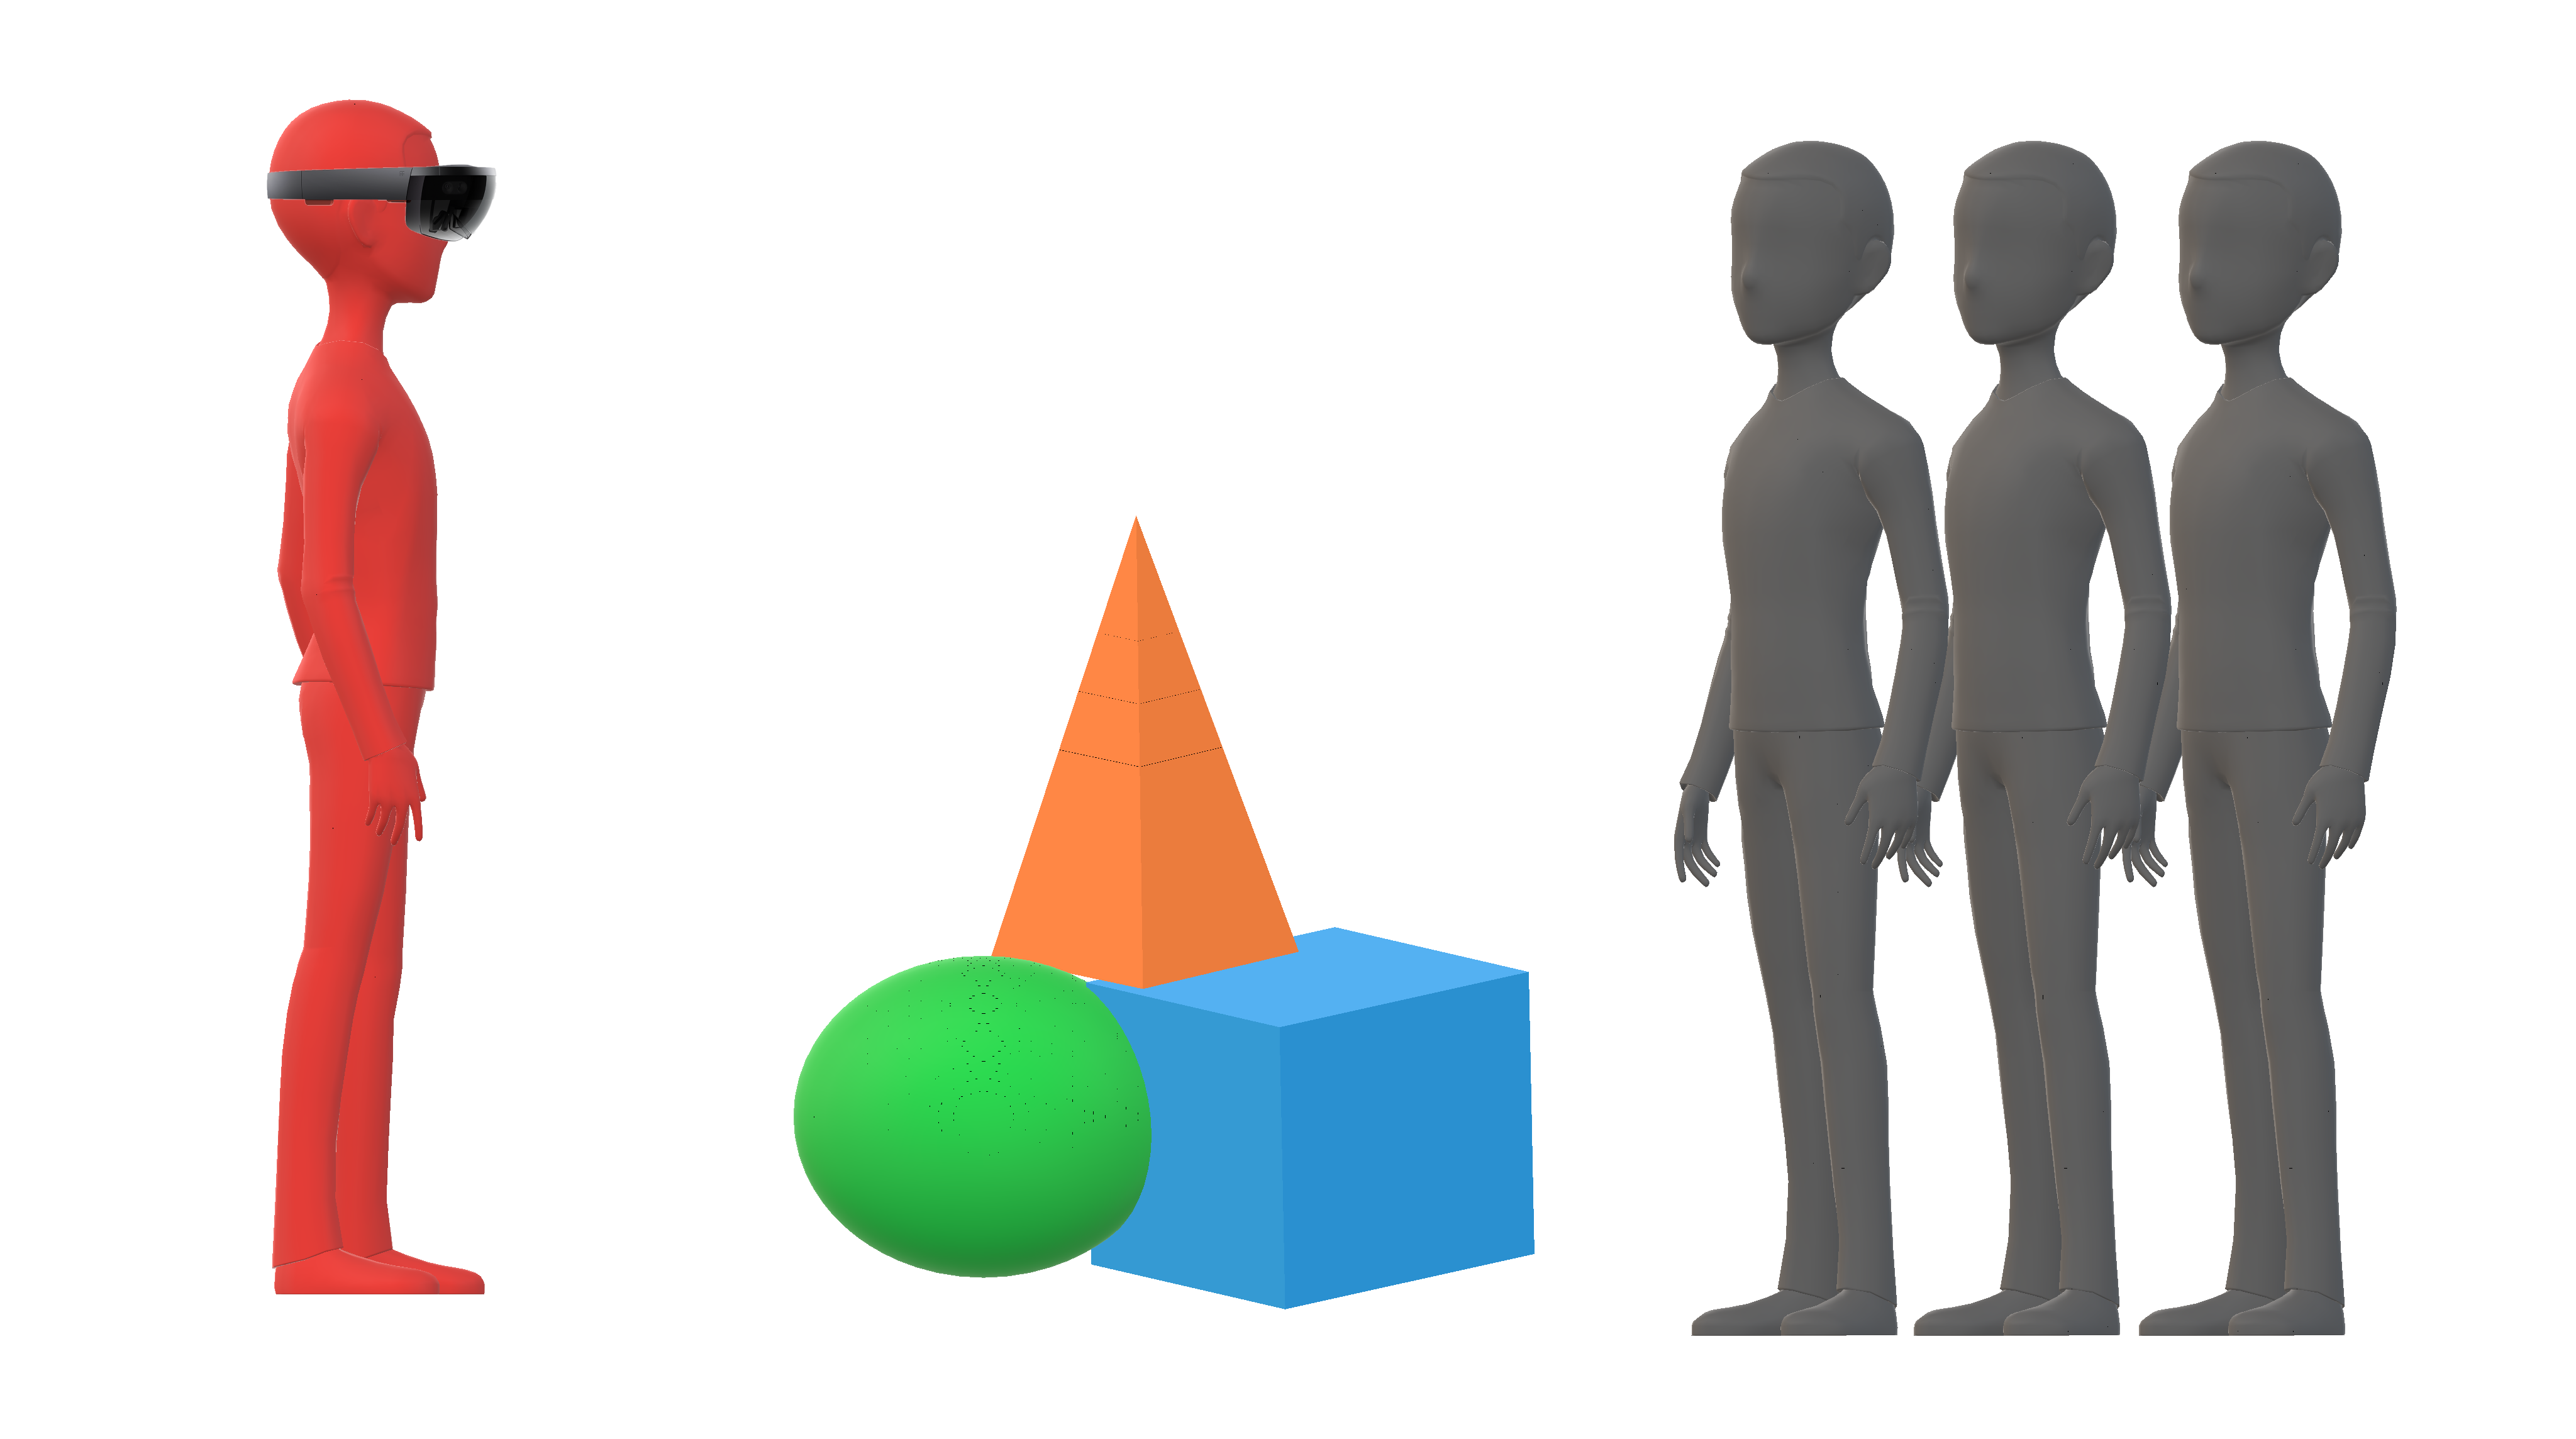
\includegraphics[width=.8\linewidth]{images/continuum_categories5.png}
    \caption{The social AR continuum categories: 1) People (self and others), 2) Objects (surrounding environment), 3) Interactions (e.g., annotations)}
    \label{fig:continuum:categories}
\end{figure}

This work aims to layout the space of the AR continuum for social sharing experiences by looking at parameters and options that can be manipulated in terms of people, objects and interactions to create a shared social AR experience. Before diving into the parameters of shared social experiences, we explore potential future scenarios where people would want to share social experiences through AR.

\section{Scenarios}

\todo[inline]{
Scenarios: 
First of all I like the graphics etc. I was even thinking if you should start with the scenarios before coming to the AR continuum. Basically, if you could use your scenarios to better motivate the need for an AR continuum?! Later you can use them again to explain some of the dimensions. In any case they are under-utilised at the moment. They need a better explanation and a better integration. For example: I would not start with the decoration one because it is the weakest one in my opinion. Maybe better start with the working from home and the social meeting. You could start with that  ….. blabla bla… explain all the things no just what is depicted in the picture…. later explain the other scenarios but similarly motivate for each scenario why this is a valid and important scenario. 
}
\todo[inline]{
Again these are all recommendations and you can take it or leave it (or take parts of it). In any case you need to integrate more references. I only put in the last part some examples on where they are needed but basically every big statement should be supported. I think this is all important because when the reader is not buying in into your scenarios, you will have a hard time selling your conceptual solutions for each scenario. The reader will simply say: The scenario is not a real scenario or is to irrelevant to be addressed by a PhD thesis as it is not solving a real problem (current and future). This is a bit the issue with the decoration scenario which is a bit random. Keep it but do not put it first.
}
\todo[inline]{
Finally, please be more verbose in your figure captions. I have the tendency to be very long (see my PhD thesis and most of my papers) but really take the space to explain what is going on in the figure and do not only provide a “figure name”. It is OK if parts are replicated in the body text. But the figure should work without the body text and the body text should work without the figure caption.
}

Let us consider the following future scenarios of sharing social AR experiences:

\subsection{Working from home}

there is increasingly support for working from home (reference needed) and AR/MR could be a key technology here to connect remote teams and people (references needed here). However, when sharing information (could be this or this or this) with remote parties we should consider also their social proximity when deciding on what to share and how to share it. Lets consider the following example where user A is working from home. He is using an AR system to share

The user is working from home and sharing their surroundings with 1) a close colleague with a few messy objects hidden/blocked, 2) a boss who sees a clean and tidy room with projection on the wall as additional augmentation, and 3) a group meeting with other workers where nothing is visible in the background. 

\begin{figure}[H]
    \centering
    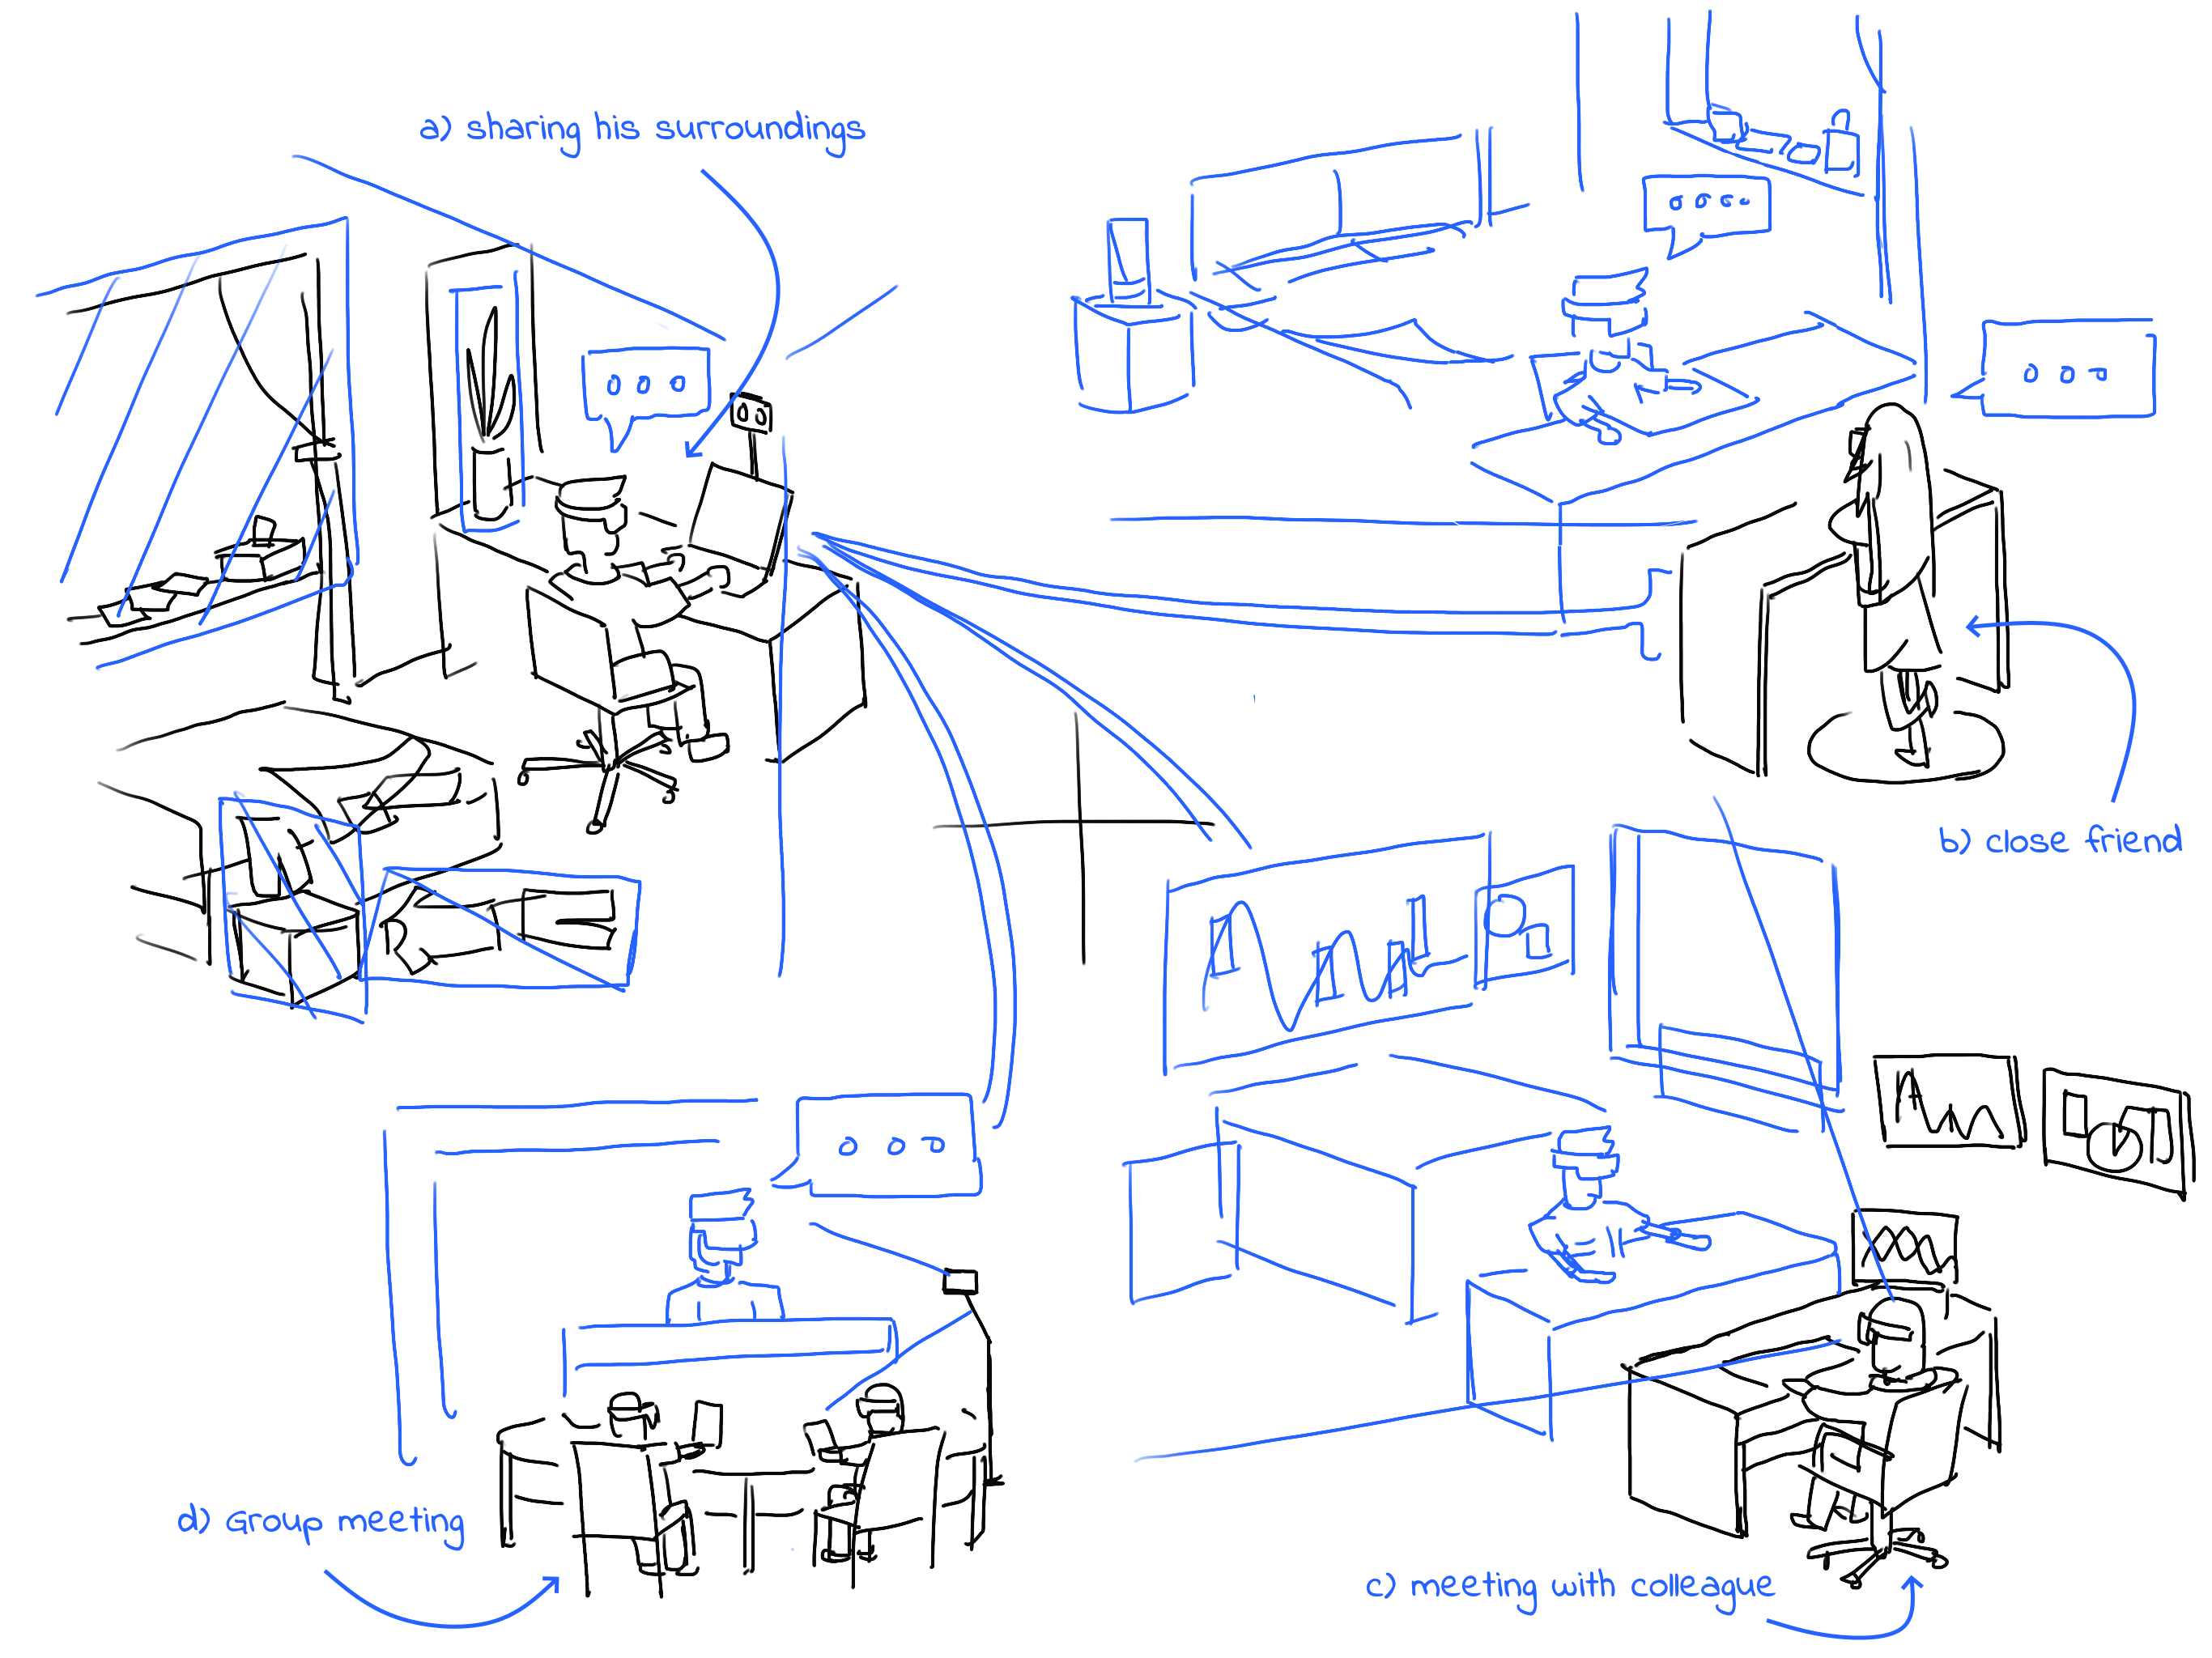
\includegraphics[width=.8\linewidth]{images/illustrations/2_Group_Meeting.png}
    \caption{Working from home (Illustrated by Kris Tong)}
    \label{fig:illustration:group-meeting}
\end{figure}

\subsection{Conference}

The user is at a conference and shares an idea that he is thinking about. However, because people around him are not close with him, they see low-fidelity details about these ideas (e.g., abstract and title). While networking with others, the user may choose to share more details about the idea  with a particular person who is in a direct conversation with him and interested in further collaboration opportunities.

\begin{figure}[H]
    \centering
    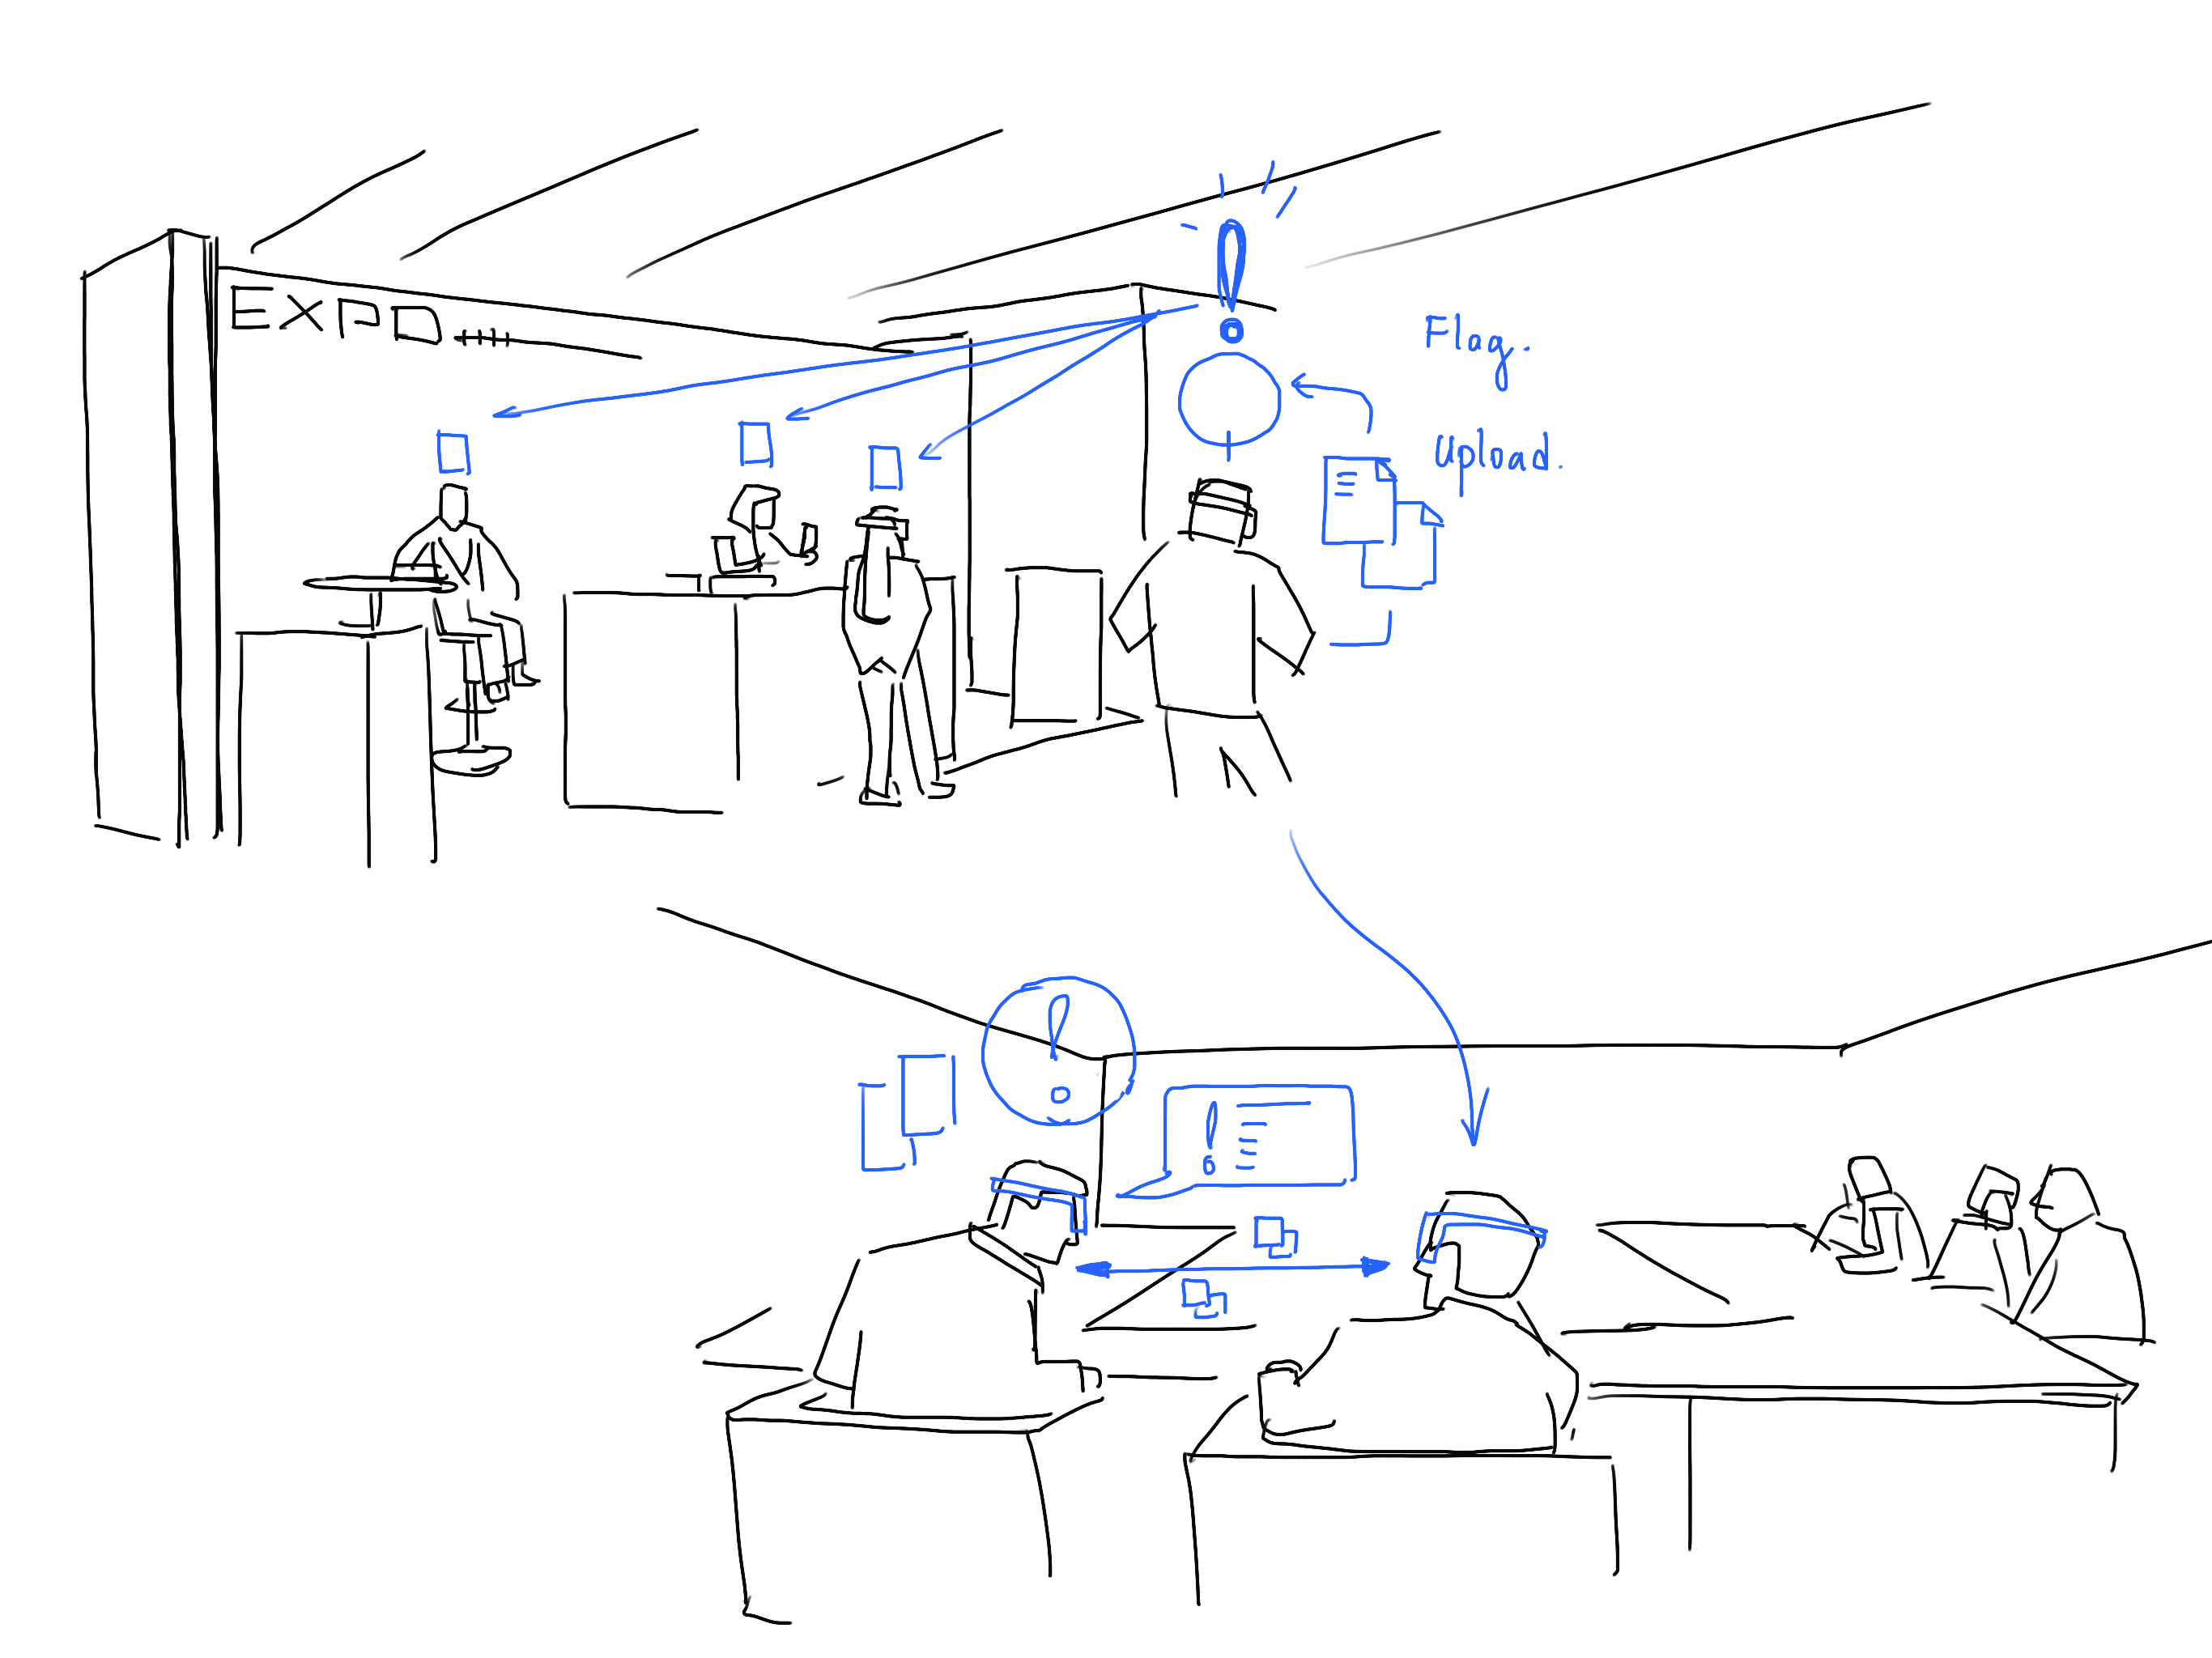
\includegraphics[width=.8\linewidth]{images/illustrations/4_Flag_On_Conference.png}
    \caption{Conference (Illustrated by Kris Tong)}
    \label{fig:illustration:conference}
\end{figure}

\subsection{Social event}

The user is at a social event where he is meeting people for a drink. He can see through their headset what their friends are sharing. For the close friends, he can see high-fidelity material such as 360-degree videos of their last trip, while for others who are less close with him he sees low-fidelity media such as 2D images. 

\begin{figure}[H]
    \centering
    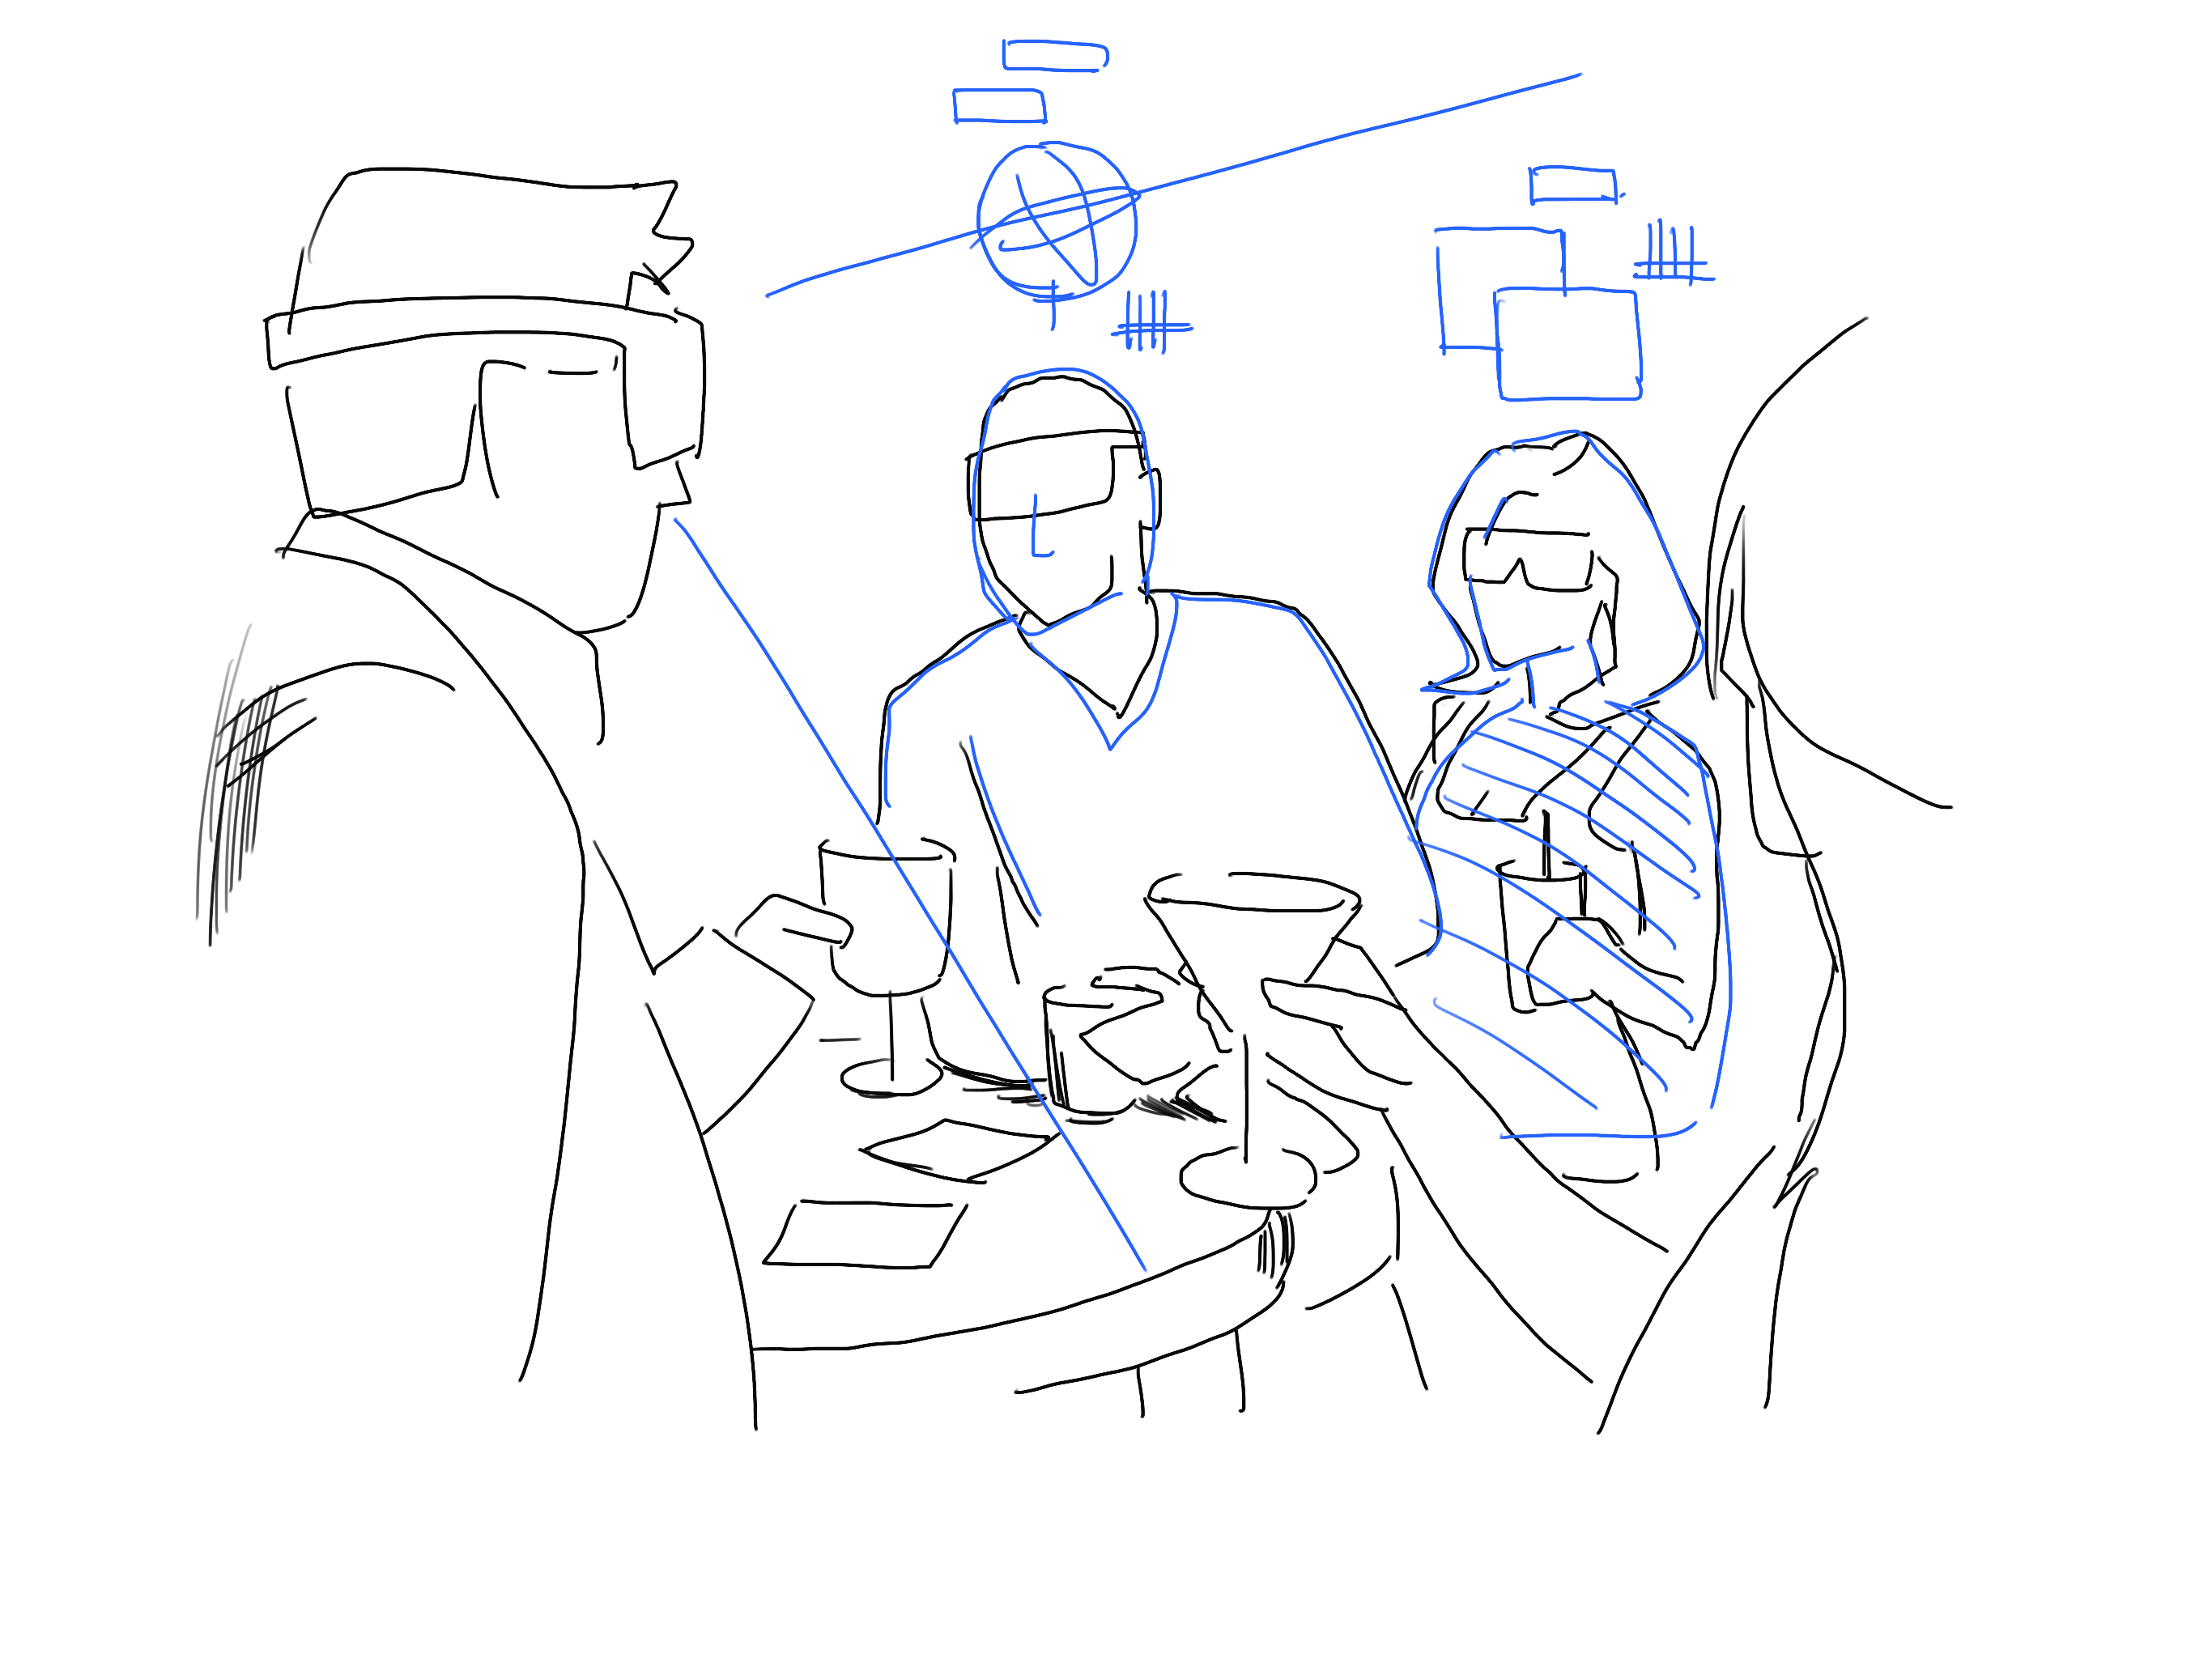
\includegraphics[width=.8\linewidth]{images/illustrations/3_Bar_Scene.png}
    \caption{Social event (Illustrated by Kris Tong)}
    \label{fig:illustration:social-event}
\end{figure}

\subsection{Collaborative decoration}

The user is sharing their room for decoration purposes with 1) a wife, 2) parents, and 3) a friend. The wife will see the full details of the room. The parents see most details, but a few items in the room are blocked/hidden. The friend will see an abstraction of the room with no details. 

\begin{figure}[H]
    \centering
    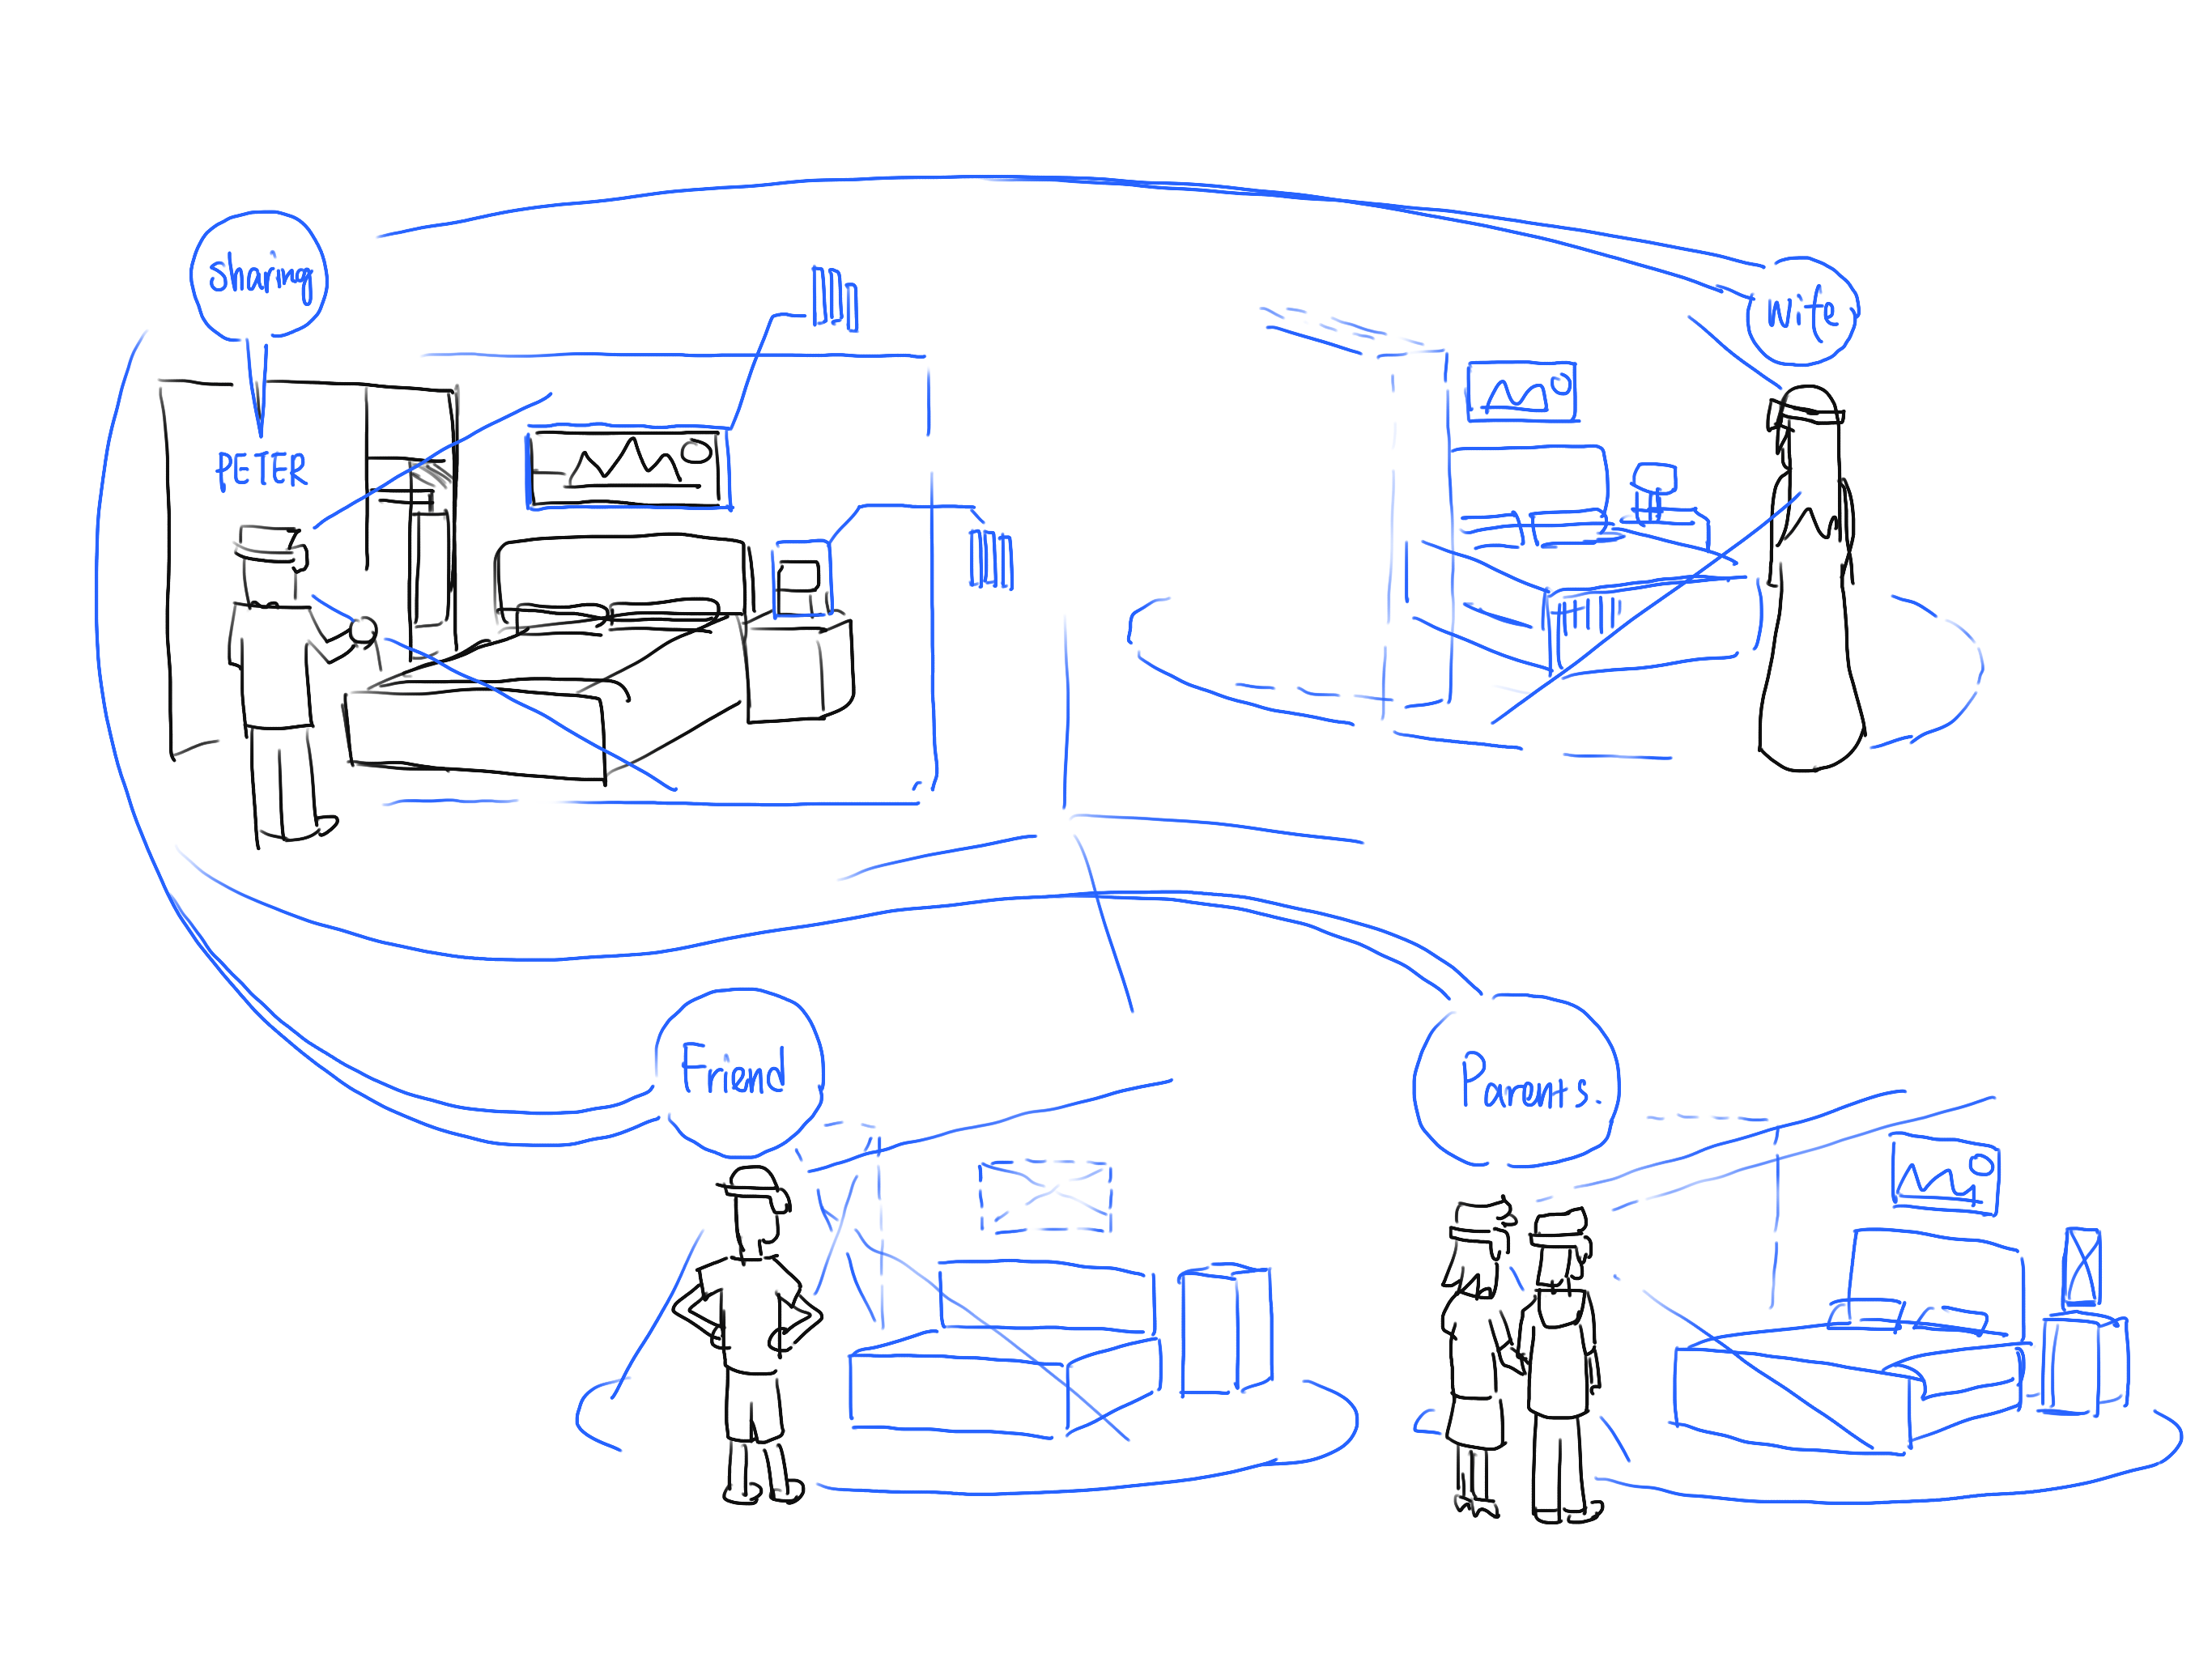
\includegraphics[width=.8\linewidth]{images/illustrations/1_Remote_Bed.png}
    \caption{Remote room decoration (Illustrated by Kris Tong)}
    \label{fig:illustration:remote-bed}
\end{figure}

\section{The Social AR continuum Dimensions}

The scenarios of social AR experiences highlighted patterns in terms of how we see others, object and interact wit them. 
Using observation from previous user studies in social AR and inspiration from continuum designs, the concept of a continuum started crystallise. 
The social AR continuum varies based on the closeness of social connections that we have with others (our relationships), and this thesis identified the following dimensions where social AR applications can fit along a continuum. The dimensions can be grouped in the categories described in Figure \ref{fig:continuum:dimensions}.

\begin{figure}[h]
    \centering
    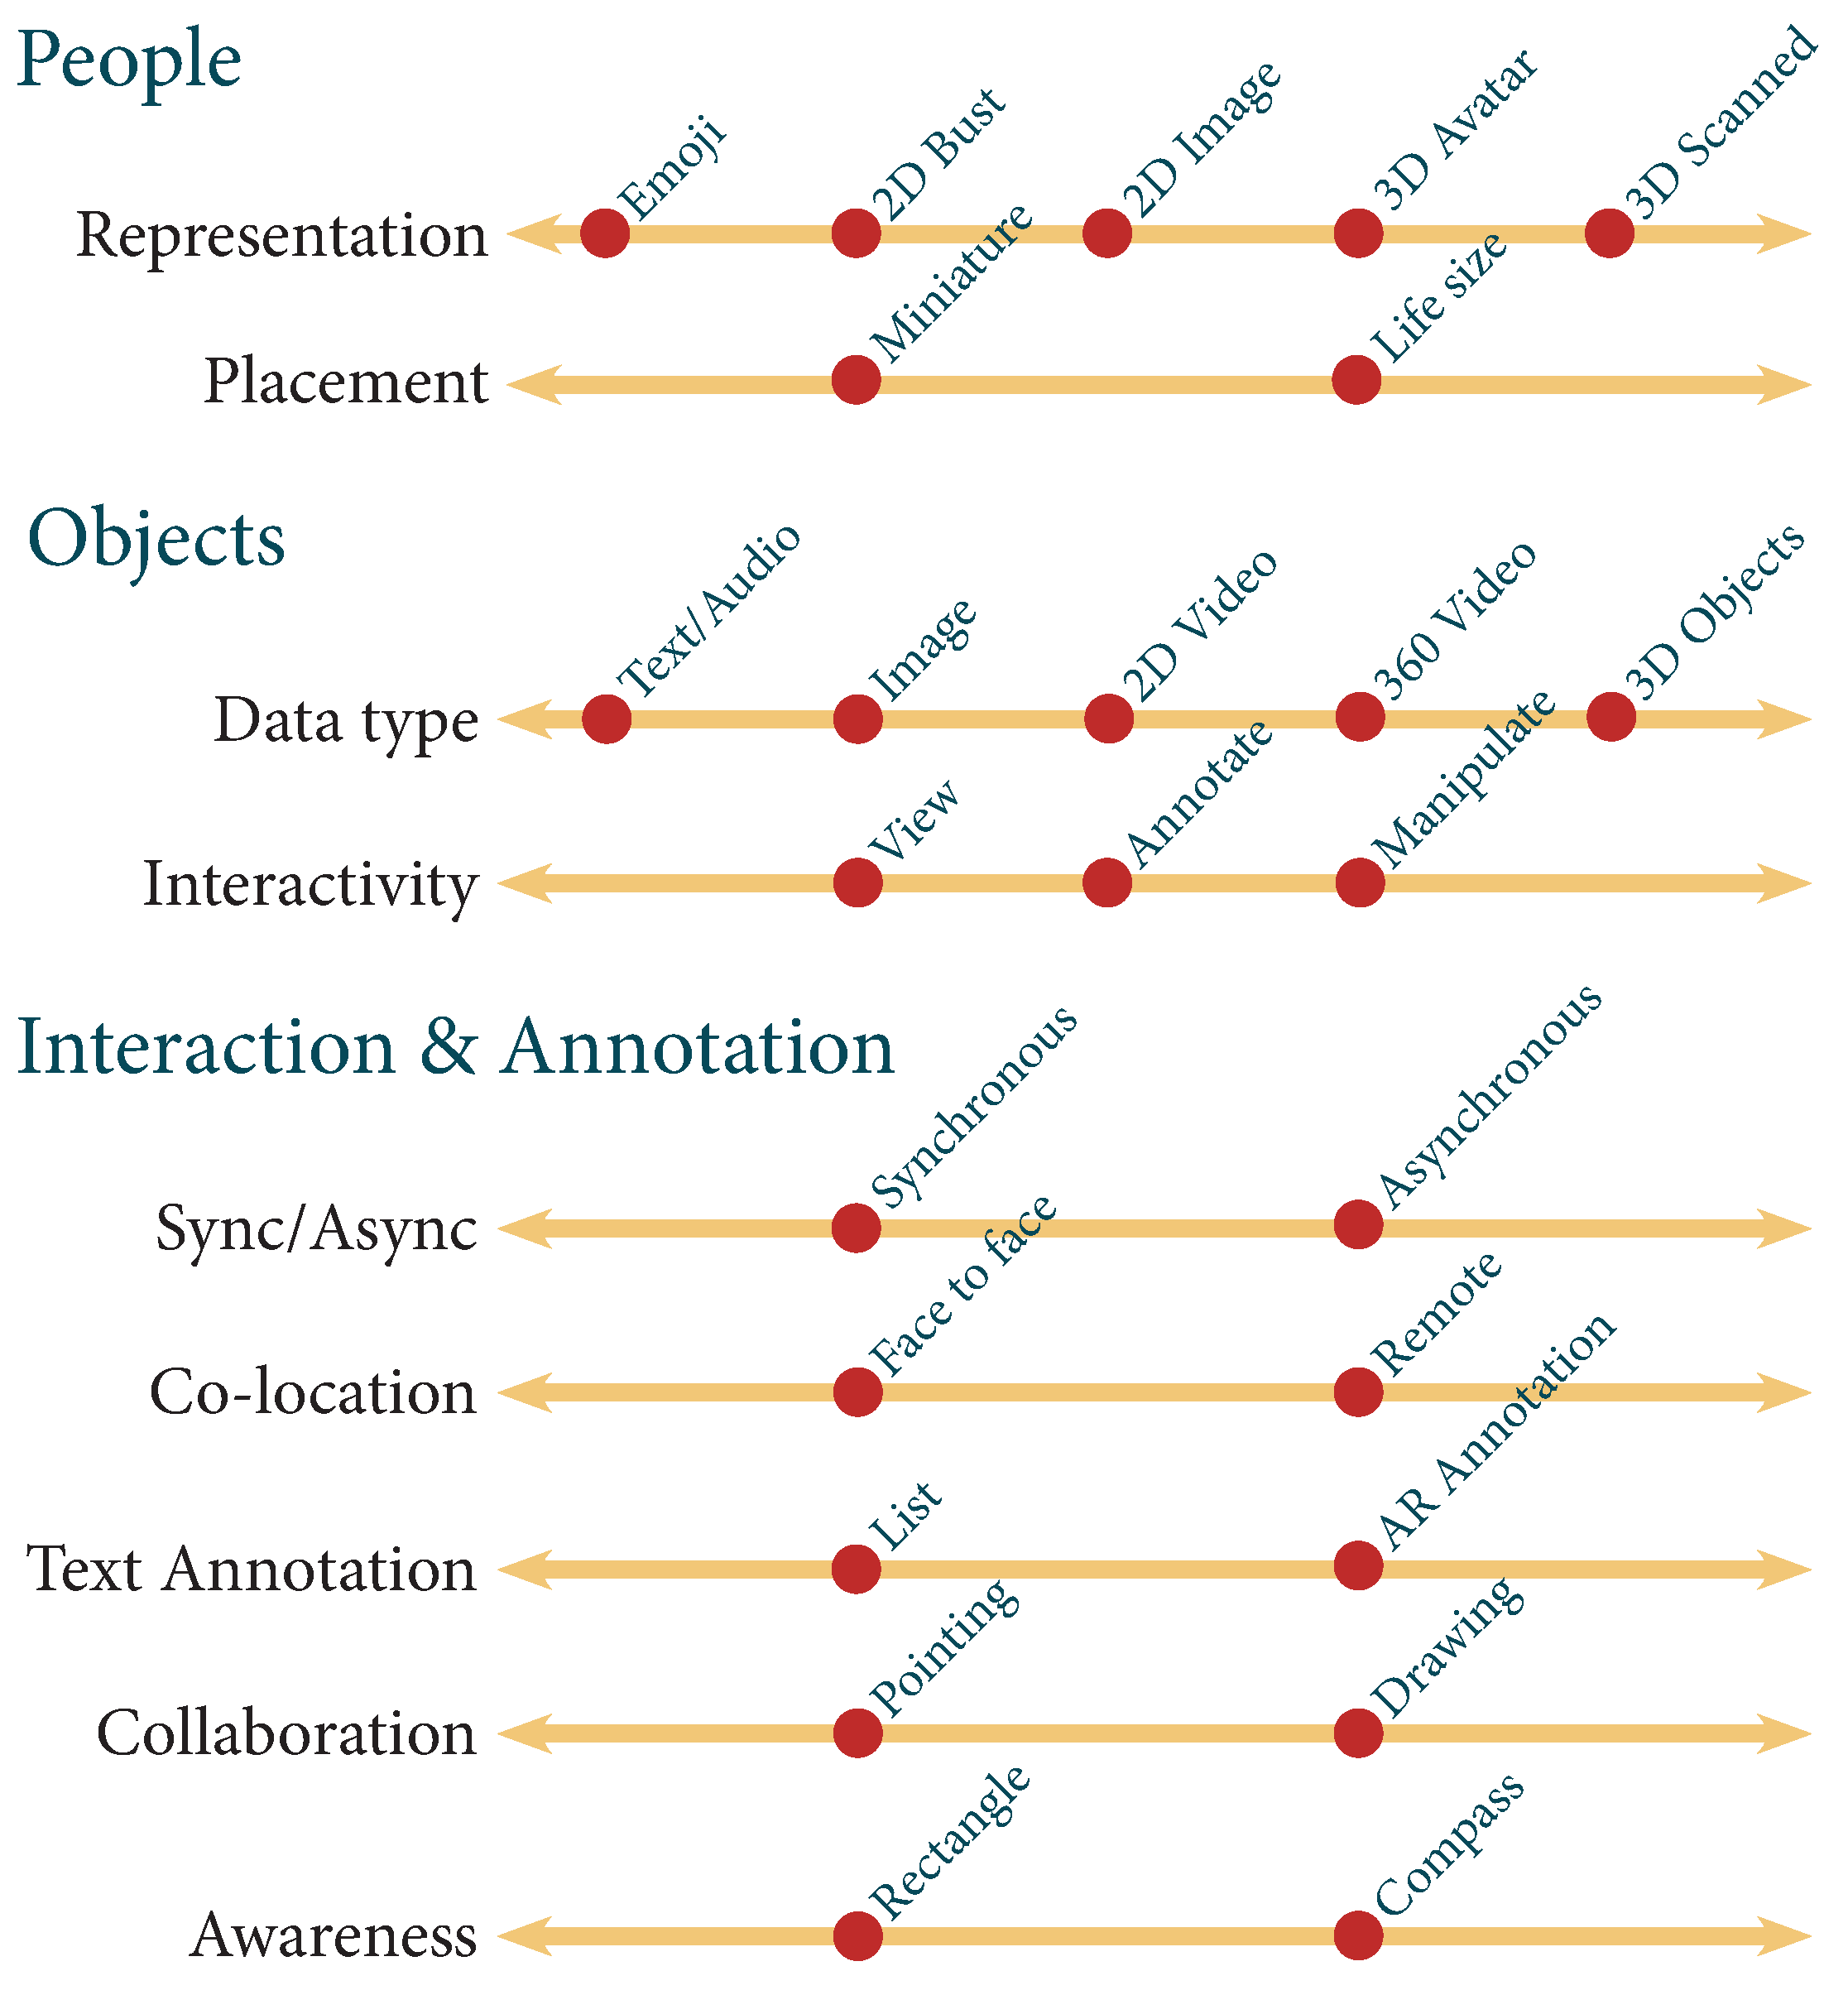
\includegraphics[width=.8\linewidth]{images/continuum4_1.eps}
    \caption{Dimensions of the social AR continuum.}
    \label{fig:continuum:dimensions}
\end{figure}

\subsection{Contact Representation}

Representing social contacts can vary on the social AR continuum based on the relationship that the user has with the contact, with closer relationships having higher fidelity. For example, \textit{Intimate} contacts could be represented as full 3D animated avatars, \textit{Friends} could be represented as 2D static images, \textit{Acquaintances} could be represented as 2D busts and \textit{Strangers} could be shown as mere emojis. Each contact could choose their representation for each category.

\begin{figure}[h]
    \centering
    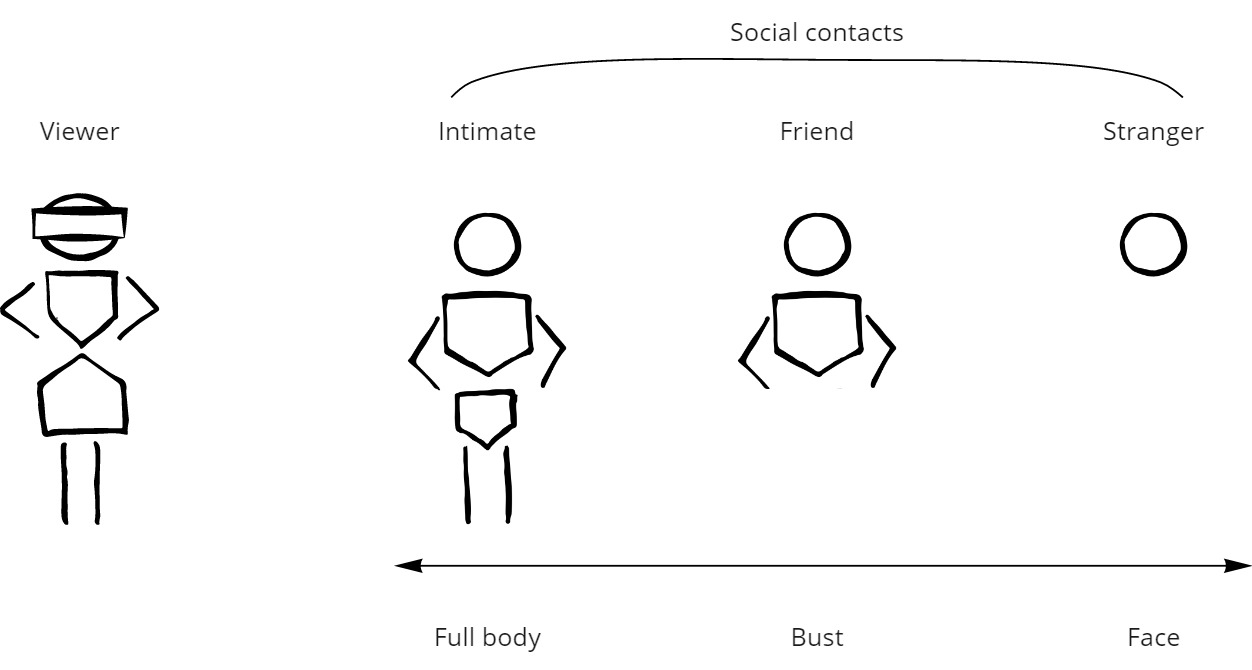
\includegraphics[width=.8\linewidth]{images/Continuum-representation.jpg}
    \caption{Contact representation}
    \label{fig:continuum:contact-representations}
\end{figure}

% \textbf{Contact Filter}
% Filtering social contacts to distinguish users from each other could be done using proximity or visual fidelity based on their relationship to the user. Proximity filters contacts by placing them closer or further away. Visual fidelity filters contacts by adding more level of detail to the contact for closer relationships and less detail for further away contacts. 

\subsection{Contact Placement}

Placing social contacts can be done either by displaying \textit{Intimates} as life-sized avatars on the ground around the user, and others as miniatures on a nearby surface. 

\begin{figure}[h]
    \centering
    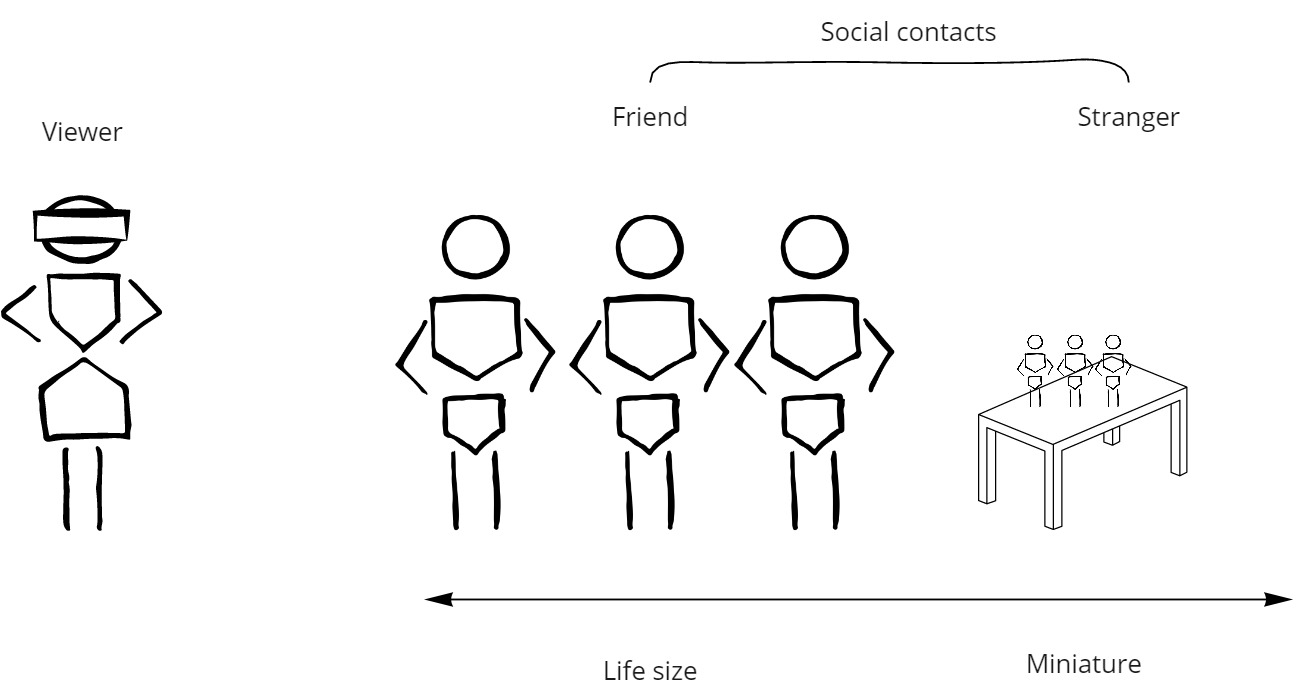
\includegraphics[width=.8\linewidth]{images/Continuum-placement.jpg}
    \caption{Contact placement}
    \label{fig:continuum:contact-placement}
\end{figure}

\subsection{Data Type}

The type of data shared between social contacts in AR could be categorised as 1D (e.g., text or audio), 2D (e.g., images, panorama or video), or 3D (e.g., 3D model or scanned-room environment). Based on the relationship between the user and their social contacts, the type of data available could be filtered. For instance, 3D data could be shared with \textit{Intimate} relationships, while \textit{Acquaintances} could see only 2D data.  

\begin{figure}[h]
    \centering
    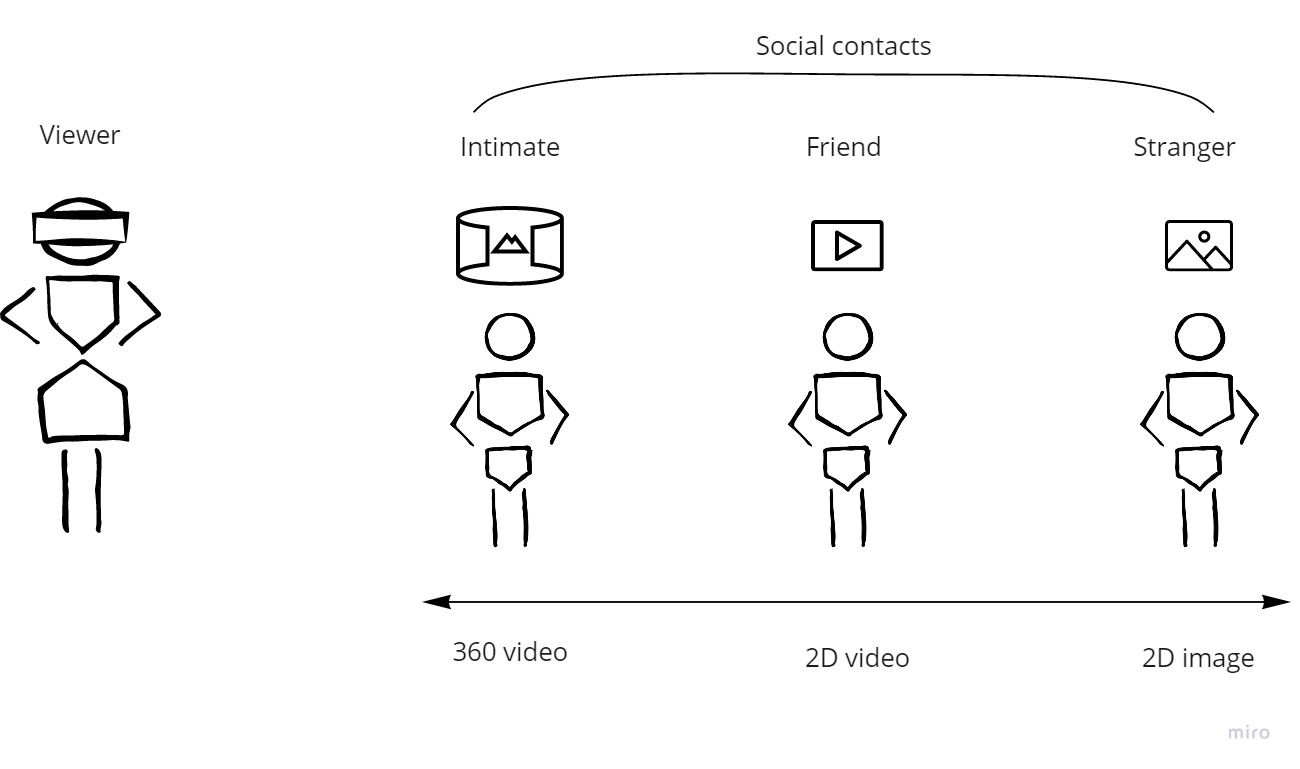
\includegraphics[width=.8\linewidth]{images/Continuum-Data-type.jpg}
    \caption{Data Type}
    \label{fig:continuum:data-type}
\end{figure}

\subsection{Data Interactivity}

In terms of user interactions with shared data, the continuum here ranges from viewing the contents, annotating or adding comments on the content, through to manipulating the content. Levels of manipulation include changing the position, rotation or scale of the shared content, or even modifying the content itself.

\begin{figure}[h]
    \centering
    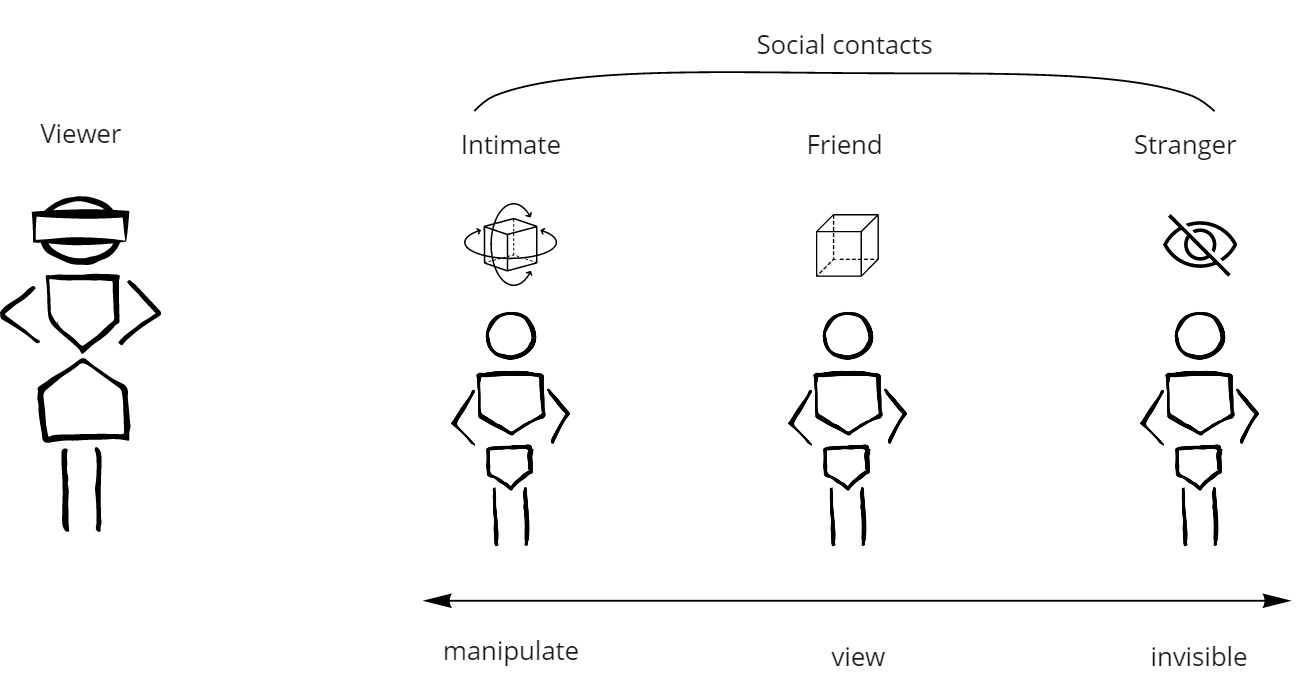
\includegraphics[width=.8\linewidth]{images/Continuum-interaction.jpg}
    \caption{Data Interactivity}
    \label{fig:continuum:data-interaction}
\end{figure}

\subsection{Data Privacy}
Based on the relationship with other users, shared data can be made private to the user, shared with specific groups of people (e.g., friends, acquaintances), or shared with everyone. This will allow users to choose the privacy levels of the shared data based on their social relationship with others. 

\subsection{Synchronous/Asynchronous Data}

The data shared with contact could be shared in a synchronous way, where both sharing and interaction happen at the same time. In contrast, data could also be shared asynchronously \cite{Smith2016}, i.e., interaction happens at a different time. 

\begin{figure}[h]
    \centering
    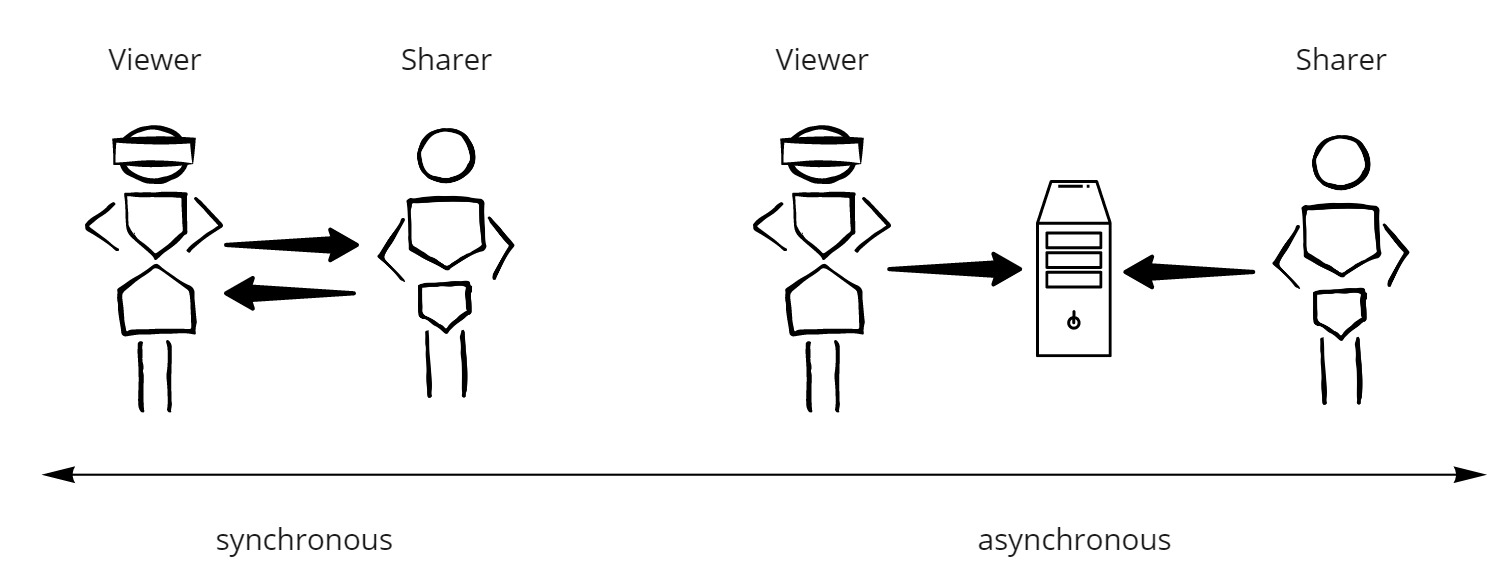
\includegraphics[width=.8\linewidth]{images/continuum-connection.jpg}
    \caption{Data Connection}
    \label{fig:continuum:data-connection}
\end{figure}

\subsection{Co-location}

Social contacts can either be remote (i.e., in a different place than the user) or face-to-face (i.e., physically in the same location as the user). When social contacts are remote, they are represented as virtual avatars based on their relationship with the user. An example of face-to-face interaction was described in a Black Mirror\footnote{http://www.imdb.com/title/tt2085059/} episode "White Christmas" where a person could 'block' another co-located person by blurring them out in their AR view of the real world.

\begin{figure}[h]
    \centering
    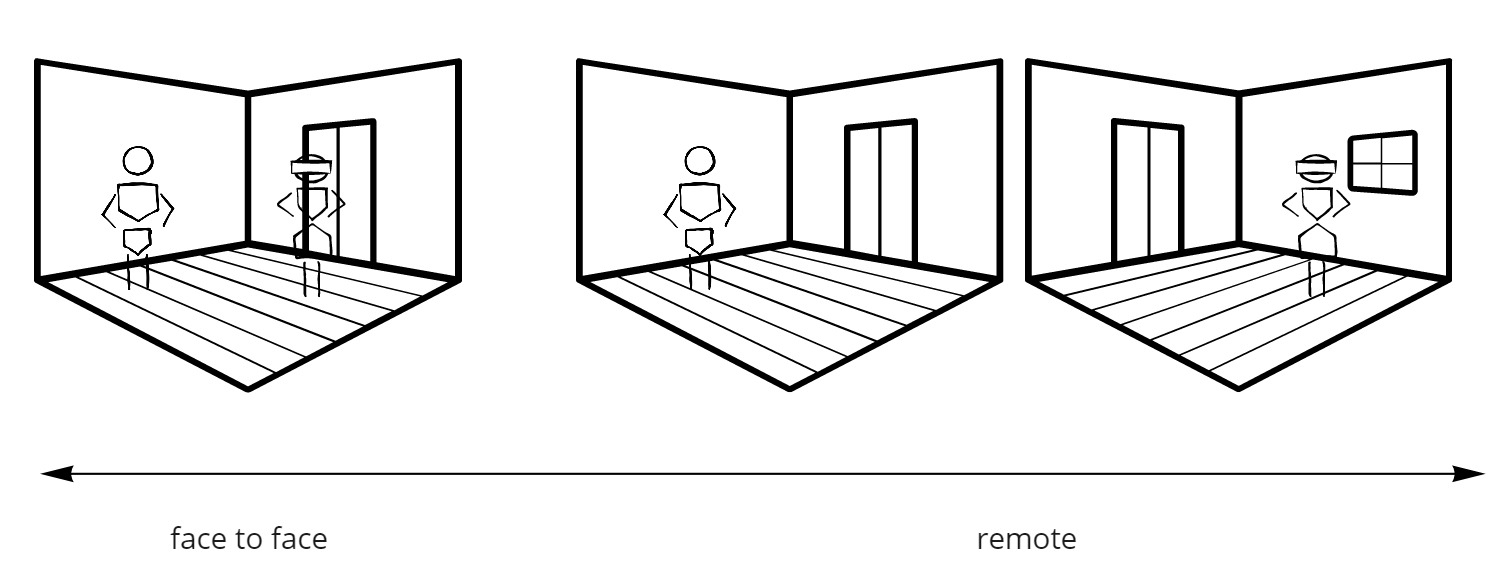
\includegraphics[width=.8\linewidth]{images/continuum-colocation.jpg}
    \caption{Data Co-location}
    \label{fig:continuum:data-colocation}
\end{figure}


\subsection{Text Annotation}

placing AR annotation or information attached to an AR object can be described as head-stabilised, body-stabilised or world stabilised \cite{Billinghurst1998}.

When adding text to describe an object or a place, the text can be placed as a list (lower fidelity) on the side of the screen or can be placed on the related object as an AR annotation (higher fidelity) that ``sticks'' to the scene and disappears if the user looks away. This dimension can be used with social contacts, and if the contact is a close friend, they would see the annotation in higher fidelity, while a stranger would see the text annotation in lower fidelity. 

% gogo: Another way to think about list vs. callouts is view-fixed (list) versus world-fixed (callouts). Feiner (I think it was him) defined a set of locations/things that text/windows could be attached to


\subsection{Collaboration}

When collaborating with social contacts, the user could use a pointer (e.g. arrow, indicator) to direct the conversation to a particular place or use a drawing tool (e.g. pencil) to highlight the area of the conversation. The availability of these options could depend on the social proximity between social contacts. If closer to each other, higher fidelity tools are available, and if strangers then the collaboration is limited to lower fidelity tools.

\subsection{Awareness}

It is possible during a session of sharing social experiences, that social contacts are looking in different directions. Awareness tools help users to know where the other user is looking. This can be achieved by showing a rectangle or a circle pointing to where the user is looking, or by using a context compass view which provides higher fidelity for closer connections.

\section{Summary}

In this work, we introduced the concept of the social AR continuum. We identified several dimensions where a social AR application could be implemented.
